\documentclass[12pt]{article}
\usepackage[utf8]{inputenc}
\usepackage[T1]{fontenc}
\usepackage{fontspec}
\usepackage{natbib}
\setmainfont{Times New Roman}
\newfontfamily\hackfont{Hack}
\usepackage{titlesec}
\usepackage{fancyhdr}
\usepackage{fancyvrb}
\usepackage{listings}
\usepackage{xcolor}
\usepackage{graphicx}
\usepackage{longtable}
\usepackage{caption}
\usepackage{hyperref}
\usepackage{setspace}
\usepackage{multirow}
\usepackage{array}
\usepackage{tikz}
\usepackage{geometry}
\usepackage{pdfpages}
\geometry{a4paper, margin=1in}
\hypersetup{colorlinks=true, linkcolor=blue, urlcolor=blue}
\renewcommand{\contentsname}{Table of Contents}

\pagestyle{fancy}
\fancyhf{} 							% Header Middle
\rhead{Lab Report}
\lhead{Technical Writing}
\rfoot{\thepage}

\begin{document}

\begin{titlepage}					% Cover Start
\begin{center}
    
\includegraphics[width=0.35\textwidth]{logo.png} \\
    \vspace{0.5cm}
    \textbf{\Huge \textcolor{teal}{NOTRE DAME} \textcolor{teal}{UNIVERSITY}} \\
    \vspace{0.5cm}
    \textbf{\Huge \textcolor{orange}{BANGLADESH}} \\
    
    \vspace{0.9cm}
    \textbf{\Huge \underline{Technical Writing Lab Report}} \\
    
    \vspace{1.5em}
    \begin{flushleft}
    	\textbf{\Large Course Code: CSE-3207} \\
		\vspace{0.3cm}        
        \textbf{\Large Course Title: Technical Writing Presentation} \\
        \vspace{0.3cm}
        \textbf{\Large Lab Task Topic: Referencing and Citation in LaTeX} \\        
    \end{flushleft}
    
    \vspace{1em}
    \begin{flushleft}
        \textbf{\Huge \textcolor{blue}{Submitted by:}} \\
        \vspace{0.3cm}
        \textbf{\Large Name: Istiak Alam} \\
        \vspace{0.3cm}
        \textbf{\Large ID: 0692230005101005} \\
		\vspace{0.3cm}        
        \textbf{\Large Batch: CSE-20} \\
        \vspace{0.5cm}
        \textbf{\Large Submission Date: }{\Large \textbf{\today}\par}
    \end{flushleft}
    \vfill
    \begin{flushleft}
        \textbf{\Huge \textcolor{blue}{Submitted to:}} \\
        \vspace{0.3cm}
        \textbf{\Large Md. Tahmid Hasan} \\
        \vspace{0.3cm}
        \textbf{\Large Lecturer,} \\
        \vspace{0.3cm}
        \textbf{\Large Notre Dame University Bangladesh}
    \end{flushleft}
\end{center}
\end{titlepage}						% Cover End

\tableofcontents
\thispagestyle{empty}
\clearpage
\pagenumbering{arabic}

\section{Lab Report-01}
\subsection{Making Document Article in Texmaker}
\textbf{Code in Texmaker :}
\begin{verbatim}
\documentclass{article}
\begin{document}
\title{Practice Lab-01 :}
\author{Istiak Alam}
\maketitle
In March 2006, Congress raised that ceiling an additional \$0.79 trillion 
to \$8.97 trillion, which is approximately 68\% of GDP. As of October 4, 
2008, the ``Emergency Economic Srabilization Act of 2008" raised the 
current debt ceiling to \$11.3 trillion.
\end{document}
\end{verbatim}
\textbf{\\ Output in Texmaker :}
\begin{figure}[h!]
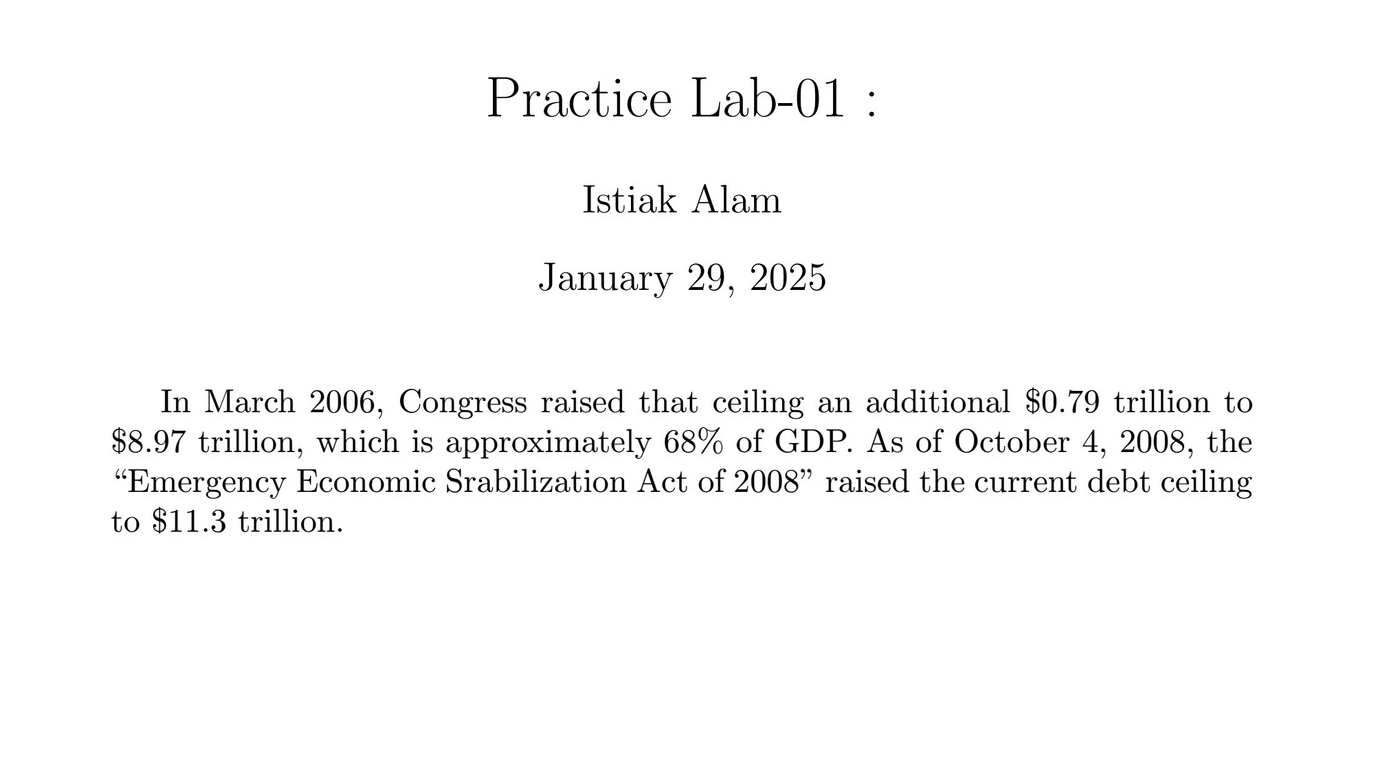
\includegraphics[width=1\textwidth]{lab1.png}
%\caption{\label{table}Output of the Article}
\end{figure}
\newpage
\section{Lab Report-02}
\subsection{Mathamatical Equation:}
\textbf{Code in Texmaker :}
\begin{verbatim}
\documentclass{article}
\begin{document}
\title{Practice Lab-02 :}
\author{Istiak Alam}
\maketitle
\textbf{Mathamatical Equation:} \\
1. $\int k\ dx = kx + C$ \\
2. $\int x^n\ dx = \frac{1}{n+1}x^{n+1}+C,\ n \neq -1 $\\
3. $\int x^{-1}\ dx = \int \frac{1}{x}\ dx = ln|x|+C$ \\
4. $\int \frac{1}{ax+b}\ dx=\frac{1}{a}ln|ax+b|+C$ \\
5. $\int ln(x)\ dx = x ln(x) -x + C $ \\
6. $\int e^x\ dx = e^x + C$ \\
7. $\int cosx\ dx = sinx + C$ \\
8. $\int sinx\ dx = -cosx + C$ \\
9. $\int sec^2x\ dx = tanx + C$ \\
10. $\int secx\ tanx\ dx = secx + C$\\ \\
11. $\int cscx\ cotx\ dx = -cscx + C$ \\ \\
12. $\int csc^2x\ dx = -cotx + C$ \\ \\
13. $\int tanx\ dx = ln|secx| + C$ \\ \\
14. $\int secx\ dx = ln|secx+tanx| + C$ \\ \\
15. $\int \frac{1}{(a^2+u^2)}\ dx = \frac{1}{a}tan^{-1}
(\frac{u}{a})+C$ \\
16. $\int \frac{1}{\sqrt[]{a^2-u^2}}\ dx = 
sin^{-1}\frac{u}{a}+C$
\end{document}
\end{verbatim}
\newpage
\textbf{Output in Texmaker :}
\begin{figure}[h!]
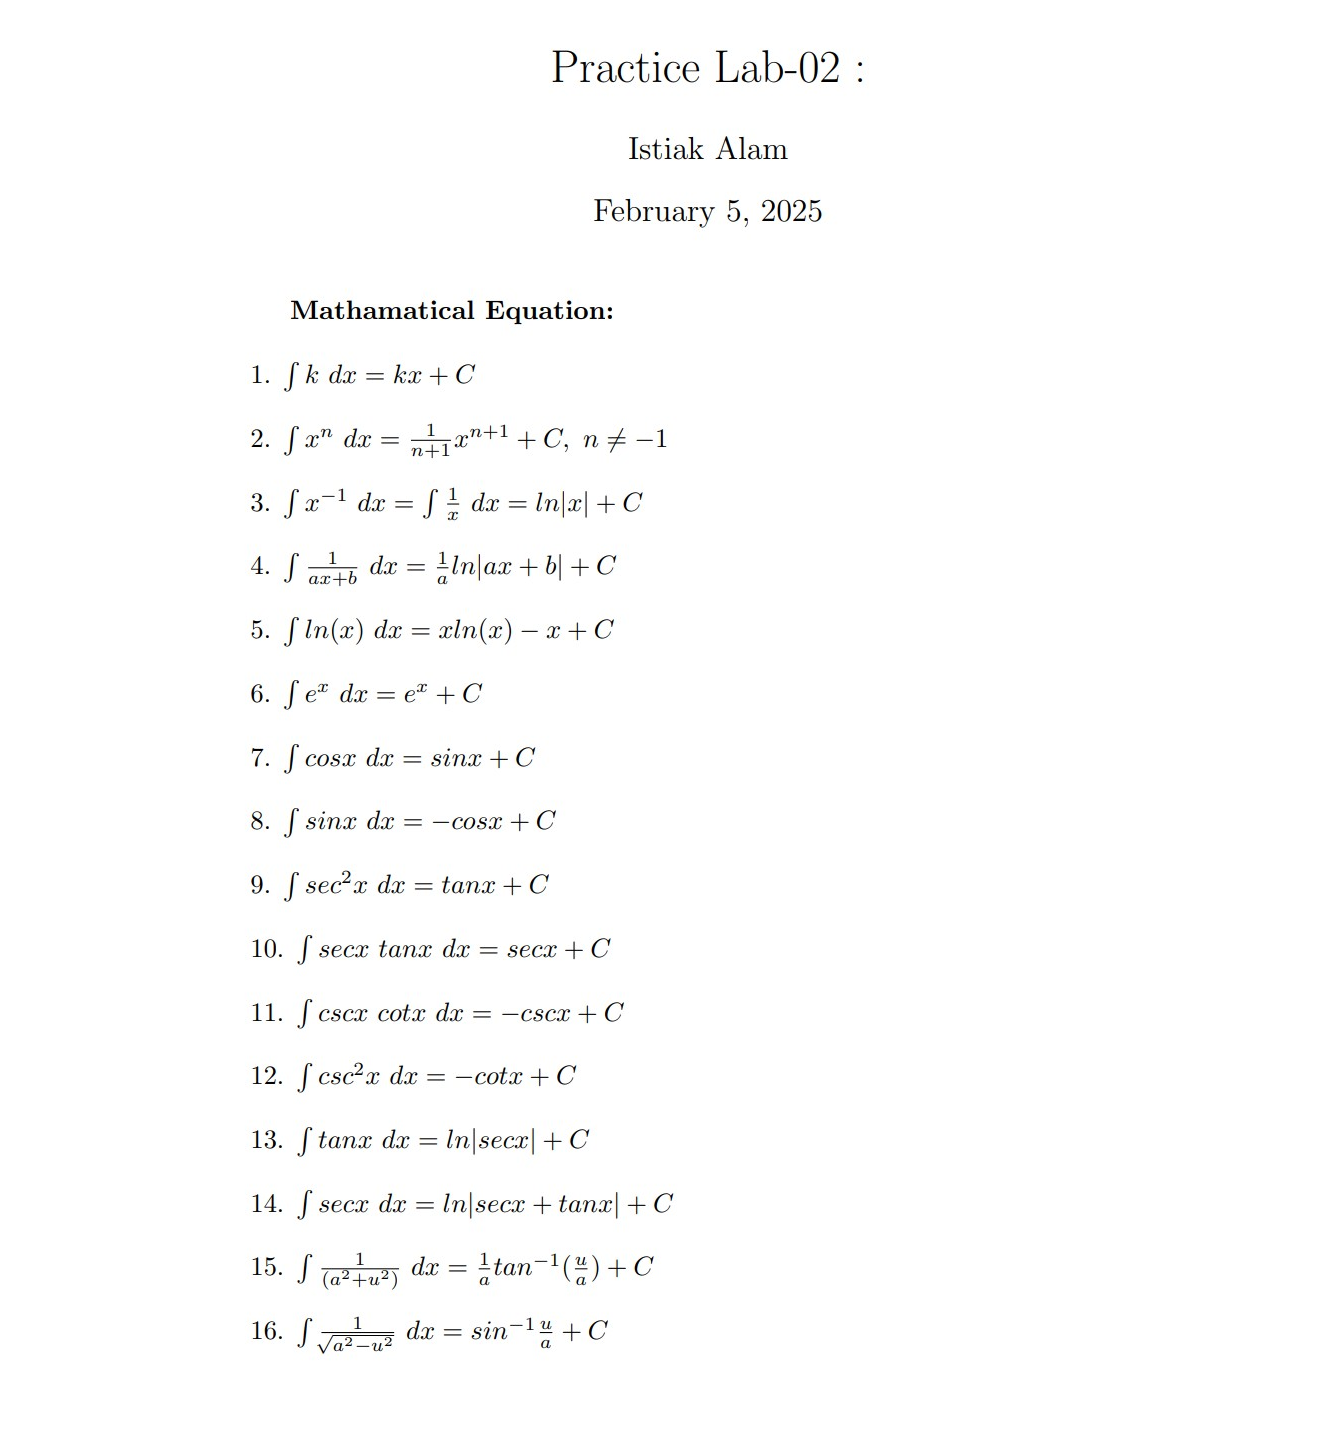
\includegraphics[width=1.1\textwidth]{lab2.png}
%\caption{\label{table}Output of the Article}
\end{figure}
\newpage
\section{Lab Report-03}
\subsection{Integral Equations :}
\textbf{Code in Texmaker :}
\begin{verbatim}
\documentclass[13pt]{article}
\begin{document}
\title{Practice Lab-03 :}
\author{Istiak Alam}
\maketitle
\textbf{Integration Properies:} \\ \\
1. $\int^b_a\ cf(x)\ dx = c \int^b_a\ f(x)\ dx$
2. $\int^b_a\ f(x) \pm g(x)\ dx = \int^a_b\ f(x)\ dx \pm \int^a_b g(x)\ dx$
3. $\int^b_a\ f(x)\ dx = 0\ and \int^b_a\ f(x)\ dx = - \int^b_a f(x)\ dx $
4. $\int^b_a\ f(x)\ dx + \int^c_b f(x)\ dx = \int^c_a f(x)\ dx$
\end{document}
\end{verbatim}

\textbf{\\ Output in Texmaker :}
\begin{figure}[h!]
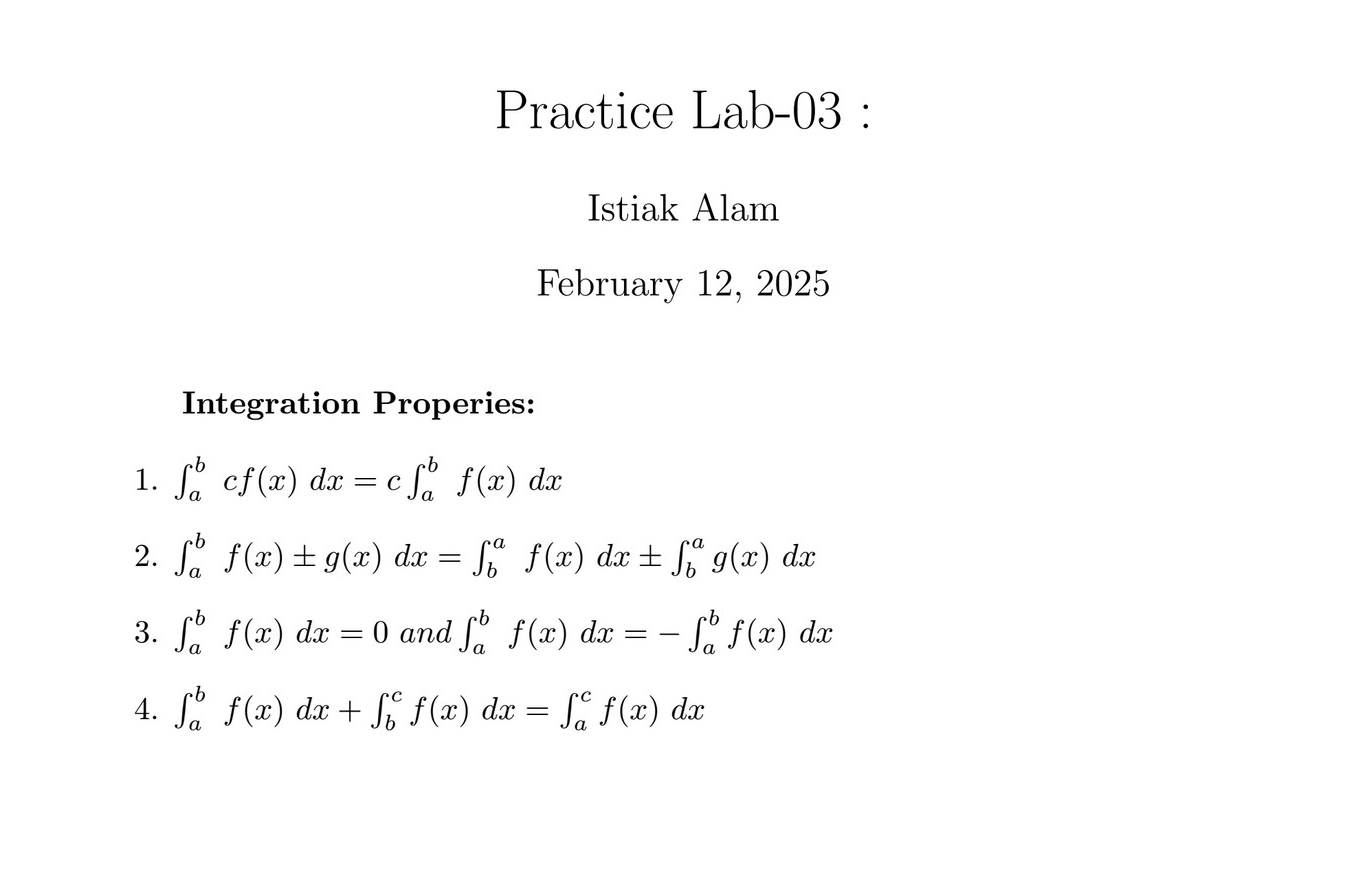
\includegraphics[width=1\textwidth]{lab3.png}
%\caption{\label{table}Output of the Article}
\end{figure}
\newpage
\section{Lab Report-04}
\subsection{Street Style `Chicken Roll' Recipe}
\textbf{Code in Texmaker :}
\begin{Verbatim}[fontsize=\footnotesize]
\documentclass[14pt]{article}
\begin{document}
\title{\underline{Lab Task-04} \\ Question-01 : Street Style `Chicken Roll' Recipe} 
\author{Istiak Alam | ID : 05}
\maketitle

\section{Ingredients of Chicken Roll}

\begin{enumerate}
    \item $\frac{1}{3}$ Cup and 2 and $\frac{1}{2}$ tablespoon chicken
    \item $\frac{1}{2}$ Medium tomato
    \item Red chilli powder as required
    \item 1 Tablespoon vegetable oil
    \item $\frac{1}{4}$ Cucumber
    \item $\frac{1}{4}$ Tablespoon coriander leaves
    \item $\frac{1}{2}$ Large onion
    \item 1 Medium green chilli
    \item 1 Pinch garam masala powder
    \item $\frac{1}{2}$ Lemon wedge
    \item $\frac{1}{2}$ Teaspoon tomato ketchup
    \item $\frac{1}{2}$ Tablespoon green chilli sauce
\end{enumerate}

\section{For Marination}
\begin{enumerate}
    \item $\frac{1}{4}$ teaspoon coriander powder
    \item Turmeric as required
    \item 1 pinch black pepper
    \item $\frac{1}{4}$ teaspoon garlic paste
    \item $\frac{1}{4}$ teaspoon cumin powder
    \item $\frac{1}{2}$ teaspoon low-fat yoghurt
    \item $\frac{1}{4}$ teaspoon ginger paste
\end{enumerate}

\section{For Dough}
\begin{enumerate}
    \item Salt as required
    \item $\frac{1}{4}$ tablespoon vegetable oil
    \item $\frac{1}{2}$ cup all-purpose flour
    \item $\frac{1}{4}$ cup water
\end{enumerate}

\section{Preparation}

\begin{itemize}
    \item For preparing this easy snack recipe, take a glass bowl and add coriander powder, 
    black pepper, garlic paste, cumin powder, low fat yoghurt, turmeric and ginger paste in it. 
    Mix well. Add the freshly washed chicken pieces in the bowl and marinate them with the 
    already added ingredients. Keep aside for minimum 1 hour or more.
\end{itemize}

\section{Cooking}
\begin{itemize}
    \item Now heat oil in a frying pan over moderate flame. Add sliced onions and saute them on
     medium flame until light brown in colour. Then add chopped tomatoes and cook for 2-3 minutes. 
     Then add the marinated chicken pieces. Mix well, cover and cook on low flame for 10 minutes. 
     Keep stirring in between. Add ½ cup of water.
    \item Cover and cook until the chicken is done, stir in between. If the chicken is drying too 
     much, sprinkle some more water. Once done add garam masala powder. Mix well and 
     remove from heat. Keep it aside.
\end{itemize}

\section{Preparing the Dough}
\begin{itemize}
    \item For the dough, mix well all purpose flower, vegetable oil and salt. Now add water 
     slowly and knead a very smooth dough. Make 3 or 4 equal sized balls out of it. On a lightly
     floured surface, roll out each ball into a round paratha (the thickness should be little 
     bit more than the regular chapatis or rotis).
\end{itemize}

\section{Cooking the Paratha}
\begin{itemize}
    \item Heat a tawa on moderate flame and cook the paratha one at a time. Flip and cook both 
    sides without oil first (cook for a minute in total), now add 1 tbsp oil for each side. 
    Flip and cook until light brown spot appears. Avoid too much flipping as the parathas may 
    get hard. Remove from heat and keep the parathas aside.
\end{itemize}

\section{Assembling the Roll}
\begin{itemize}
    \item Now on a hot paratha, arrange some cooked chicken pieces in a row (make this line little
     apart from the center). Drizzle some lemon juice all over the chicken pieces, garnish with 
     some sliced onions, cucumber and chopped coriander leaves. Add few drops of tomato ketchup
     and chili sauce.
    \item Roll the paratha firmly and wrap one half of the roll with tissue paper. Fold the bottom
     part of the tissue paper inside the roll. Your street style ‘Chicken Roll’ is ready to eat. 
     Enjoy!
\end{itemize}

\end{document}
\end{Verbatim}

\section{Lab Report-05}

\section{Lab Report-06}

\section{Lab Report-07}

\section{Lab Report-08}

\end{document}